% Conference paper (IEEE two-column format, as used by ISBI and other IEEE imaging venues).
% Tables under tables/ are generated by `make tables` and `make gradcam`; figures are read from
% ../reports/figures. Every number in the prose comes from reports/results.md,
% reports/results_macro.csv or reports/gradcam_boxes.md. Build with `make paper` from the
% repository root.
\documentclass[conference]{IEEEtran}
\usepackage[T1]{fontenc}
\usepackage{cite}
\usepackage{graphicx}
\usepackage{booktabs}
\usepackage{amsmath}
\usepackage[hidelinks]{hyperref}
\graphicspath{{../reports/figures/}}

\begin{document}

\title{Do Frozen Chest X-ray Foundation-Model Embeddings Transfer Across Hospitals Better Than a Fine-Tuned CNN?}

\author{%
\IEEEauthorblockN{Shaya Arya}
\IEEEauthorblockA{Master's in Artificial Intelligence\\Universitat de Barcelona, Barcelona, Spain}}

\maketitle

\begin{abstract}
We ask whether frozen medical vision foundation-model embeddings transfer across hospitals better than a fully fine-tuned convolutional network, and whether retrieval-based prediction ($k$-nearest-neighbour voting over an embedding index) degrades less under distribution shift than a trained linear head. On NIH ChestX-ray14 (112,120 images) and the Indiana University collection (3,603 images), with a shared six-label space, patient-level splits and 1,000-resample patient-level bootstrap intervals, we evaluate four frozen encoders (RAD-DINO, BiomedCLIP, DINOv2 and an ImageNet ResNet-50) with linear-probe and $k$NN heads at 1\%, 10\% and 100\% of the source labels, against an end-to-end fine-tuned ResNet-50 on the same cells. Three findings. The in-distribution-minus-out-of-distribution gap is dominated by how hard each test split is, so we report the shortfall against an in-domain model on the same test set with paired intervals. Retrieval loses less of its in-domain ceiling under transfer than the probe does, but its ceiling is lower, so the probe remains the better transferred model in most settings. With 78k source labels the fine-tuned network ties the best frozen pipeline (macro AUROC 0.814 vs 0.815 on NIH, 0.877 vs 0.869 on IU); with 2.6k labels it trails the RAD-DINO probe by 0.07 to 0.12 AUROC and shows the largest transfer shortfall of any model, while localising radiologist boxes far better than the frozen probe (pointing game 0.45 vs 0.22). All code, splits and cached embeddings reproduce every number. No clinical utility is claimed.
\end{abstract}

\begin{IEEEkeywords}
chest radiography, foundation models, distribution shift, retrieval, calibration
\end{IEEEkeywords}

\section{Introduction}

Deep classifiers for chest radiographs lose performance when moved to a hospital they were not trained in~\cite{zech2018,pooch2020}. Frozen image encoders pretrained on large radiology corpora~\cite{perezgarcia2025,zhang2025biomedclip} promise a different workflow: compute one embedding per image, train a small head on whatever labels a site has, and keep the encoder fixed. Two questions follow for anyone deploying such a pipeline. Does a head on frozen features survive a change of hospital better than a network fine-tuned end to end on the same labels? And does predicting by retrieval, voting over the nearest labelled training images, degrade less than a trained linear head, as retrieval has no weights that can overfit the source site?

We answer both on two public datasets whose differences are typical of a cross-hospital move: NIH ChestX-ray14~\cite{wang2017}, large and labelled by report mining, and the Indiana University (Open-i) collection~\cite{demnerfushman2016}, small and labelled by hand. Contributions:
\begin{enumerate}
  \item A leave-one-dataset-out protocol over four frozen encoders, two head families, three label regimes and a fine-tuned baseline, with patient-level splits and patient-level bootstrap intervals shared across every model so that comparisons are paired (Section~\ref{sec:protocol}).
  \item Evidence that the common ``in-distribution minus out-of-distribution'' gap is confounded by test-set difficulty on these datasets, and a same-test-set transfer gap that is not (Section~\ref{sec:results}).
  \item A quantitative answer: retrieval degrades less but from a lower ceiling; frozen medical encoders win when source labels are scarce and only tie fine-tuning when they are plentiful; and fine-tuning buys localisation (Section~\ref{sec:results}).
\end{enumerate}
The question matters beyond benchmarking. A clinic or a research group with a few thousand labelled radiographs and no training cluster can run the frozen-embedding workflow on a laptop; whether it should, and whether retrieval or a trained head is the safer choice when the images come from elsewhere, is what this paper measures.

\section{Related work}

\paragraph{Cross-hospital shift in chest radiography}
Zech et al.~\cite{zech2018} showed that a pneumonia classifier trained on radiographs from two hospital systems performed worse on a third, and that the network could tell the source hospital from the image. Pooch et al.~\cite{pooch2020} and Cohen et al.~\cite{cohen2020limits} measured the same drop across the public chest X-ray collections and found it the rule rather than the exception, with part of it traceable to what each collection means by a label. ChestX-ray14 is labelled by report mining, and Oakden-Rayner~\cite{oakdenrayner2020} documented how often those labels disagree with the images. The larger collections with their own label pipelines, CheXpert~\cite{irvin2019}, MIMIC-CXR~\cite{johnson2019mimic} and VinDr-CXR~\cite{nguyen2022vindr}, are the usual test beds for such studies; all three require credentialed access, which is why this paper uses the two public collections that do not.

\paragraph{Pretrained encoders and how to adapt them}
Transfer from ImageNet is the default recipe for chest radiographs, and Ke et al.~\cite{ke2021chextransfer} found that ImageNet accuracy predicts little about downstream chest X-ray performance once a network is fine-tuned. Radiology-specific pretraining changes the picture: REMEDIS~\cite{azizi2023} reported that self-supervised medical encoders transfer out of distribution with far fewer labels, RAD-DINO~\cite{perezgarcia2025} showed that image-only self-supervision on chest X-rays matches text-supervised models, and BiomedCLIP~\cite{zhang2025biomedclip} and ConVIRT~\cite{zhang2022convirt} learn from paired images and text. Whether to freeze such an encoder or fine-tune it is itself an open question. Kumar et al.~\cite{kumar2022finetuning} showed on natural-image benchmarks that fine-tuning can distort pretrained features and underperform a linear probe out of distribution while beating it in distribution, and Kornblith et al.~\cite{kornblith2019} that ImageNet accuracy predicts fine-tuned transfer far better than it predicts the quality of fixed features. This paper measures both regimes on the same patient splits in a medical setting.

\paragraph{Retrieval, calibration and localisation}
$k$-nearest-neighbour classification over frozen features is the standard label-efficient probe of self-supervised representations~\cite{caron2021} and has been argued to be a competitive classifier in its own right when the index is large~\cite{nakata2022}; exact search over a hundred thousand vectors is cheap with FAISS~\cite{johnson2019}. We report expected calibration error as used by Guo et al.~\cite{guo2017}. For localisation we use class activation maps~\cite{zhou2016}, which coincide with Grad-CAM~\cite{selvaraju2017} for networks that end in global average pooling, and score them with the pointing game of Zhang et al.~\cite{zhang2018pointing} and the energy-based measure of Score-CAM~\cite{wang2020scorecam} against the radiologist boxes released with ChestX-ray14~\cite{wang2017}.

\section{Data and protocol}
\label{sec:protocol}

\paragraph{Datasets and labels}
NIH ChestX-ray14 provides 112,120 frontal radiographs of 30,805 patients with fourteen report-mined labels. The IU collection pairs each radiology report with manually assigned MeSH terms; after dropping the 86 reports that were never indexed, 3,603 frontal images remain. Both are mapped to a shared label space of five pathologies (atelectasis, cardiomegaly, consolidation, pleural effusion, pneumothorax) plus ``no finding''; findings outside the set count as negatives, and each dataset's own normal label is kept as ``no finding''. In IU, ``cardiac shadow/enlarged'' maps to cardiomegaly and hydro- or hemopneumothorax to pneumothorax. Consolidation (30 images) and pneumothorax (27) are rare in IU, which widens every interval involving them. Images are cached once as 8-bit grayscale PNGs with the shortest side at 518 pixels.

\paragraph{Splits}
Splits are by patient. NIH keeps its official test list (25,596 images of 2,797 patients) and carves 10\% of the remaining patients for validation (train 78,124, validation 8,400). IU ships no patient identifier, so each report is treated as its own patient; 20\% of reports form the test split (721) and 10\% of the rest the validation split (288), leaving 2,594 for training. The official NIH test list is skewed relative to its training pool (39\% vs 22\% of images with any of the five pathologies; 57\% vs 35\% anterior--posterior views), which matters for Section~\ref{sec:gapdef}.

\paragraph{Label regimes}
A source model may use 1\%, 10\% or 100\% of the source training labels; subsets are whole patients drawn with three seeds, and the validation split is subsampled at the same fraction so that model selection never sees more labels than training. For NIH we add a ``matched'' regime with as many images as IU's full training split (2,594), which separates the effect of training-set size from that of the hospital.

\paragraph{Metrics and intervals}
We report AUROC, AUPRC and expected calibration error (ECE, 15 equal-width bins) per label, and the macro over the five pathologies. Intervals are 95\% percentile intervals from 1,000 bootstrap resamples of \emph{patients}; the same resampled patients are used for every model on a given test split, so differences between models are evaluated on identical resamples and their intervals are paired. Point estimates are from the first seed; the spread of the point estimate over seeds is reported separately.

\section{Models}

\paragraph{Frozen encoders}
RAD-DINO (ViT-B/14, 518-pixel input, CLS token, 768-d)~\cite{perezgarcia2025}, BiomedCLIP's image tower (ViT-B/16, projected 512-d)~\cite{zhang2025biomedclip}, DINOv2 ViT-B/14 (768-d)~\cite{oquab2024} and an ImageNet ResNet-50 (global-average-pooled 2048-d)~\cite{he2016}, each at its native preprocessing. Every image is embedded once; all heads run on the cached arrays. The public RAD-DINO checkpoint was pretrained on all of ChestX-ray14 (without labels) as well as CheXpert and MIMIC-CXR, so IU is the only dataset unseen by every encoder.

\paragraph{Heads}
The \emph{linear probe} is one $L_2$-regularised logistic regression per label on standardised embeddings, with the regularisation strength chosen on the source validation split from $\{10^{-4},\dots,1\}$ by macro AUROC. The \emph{retrieval head} is an exact cosine $k$-nearest-neighbour index (FAISS flat inner product over unit-normalised embeddings~\cite{johnson2019}); a test image's score for a label is the fraction of its $k$ nearest training images that carry the label, $k\in\{5,20,50\}$, clipped to the index size.

\paragraph{Fine-tuned baseline}
The same ResNet-50, initialised from ImageNet, with every layer trained by binary cross-entropy over the six labels (AdamW, learning rate $10^{-4}$, batch 64, random resized crops and $\pm10^\circ$ rotations, learning rate divided by ten on a validation plateau, early stopping on validation macro AUROC). It is trained on exactly the same patient subsets as the frozen heads and evaluated with the frozen ResNet-50's transform, so the two differ only in whether the weights moved. The 78k-image run took 3.7 hours on a laptop GPU (best of six epochs).

\paragraph{Localisation}
ChestX-ray14 ships 984 radiologist boxes on 880 test images; 577 are for labels in our set (none for consolidation); one falls outside the centre crop, leaving 576. For a network ending in global average pooling and a linear layer, Grad-CAM~\cite{selvaraju2017} at the last convolutional block equals the class activation map~\cite{zhou2016}, so we compute it in closed form from the output weights, and for the frozen encoder from the probe's coefficients divided by the standardiser's scale. We score the pointing game (map maximum inside the box) and the fraction of map energy inside the box~\cite{wang2020scorecam}, each next to what a uniform map would score (the box's area fraction), on the same boxes and resamples for every model.

\begin{figure*}[!t]
  \centering
  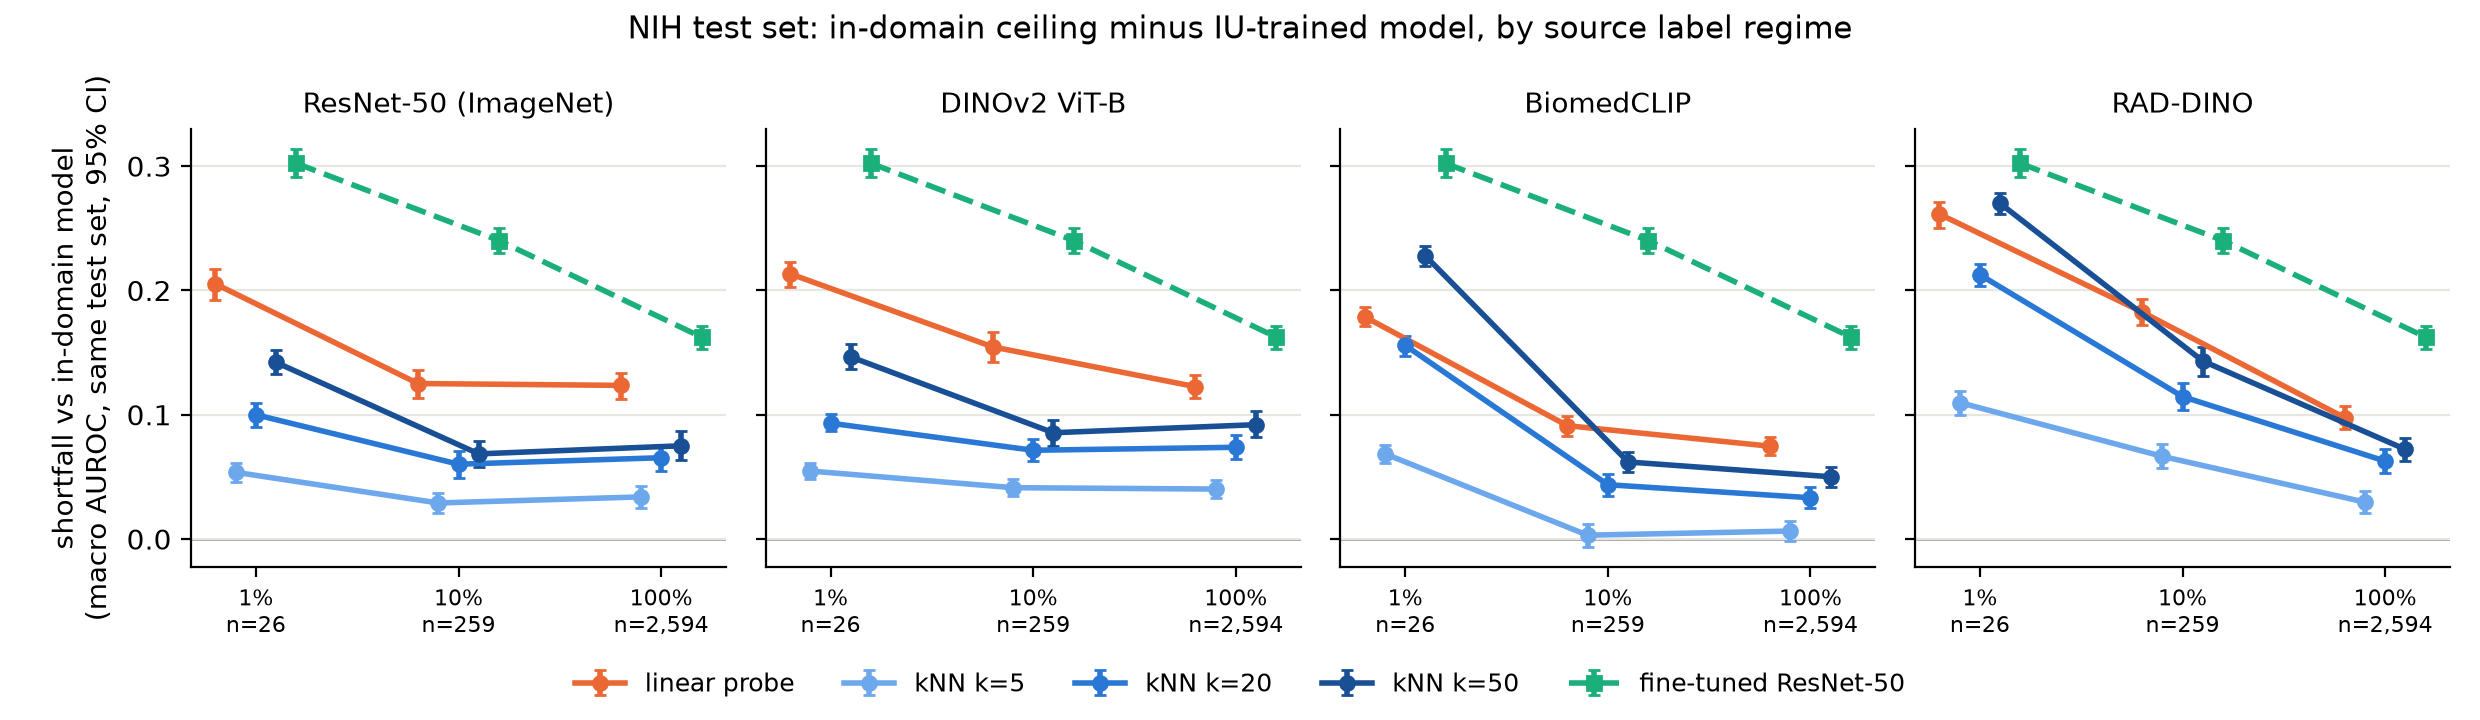
\includegraphics[width=\textwidth]{transfer_auroc_target_nih.png}\\[2pt]
  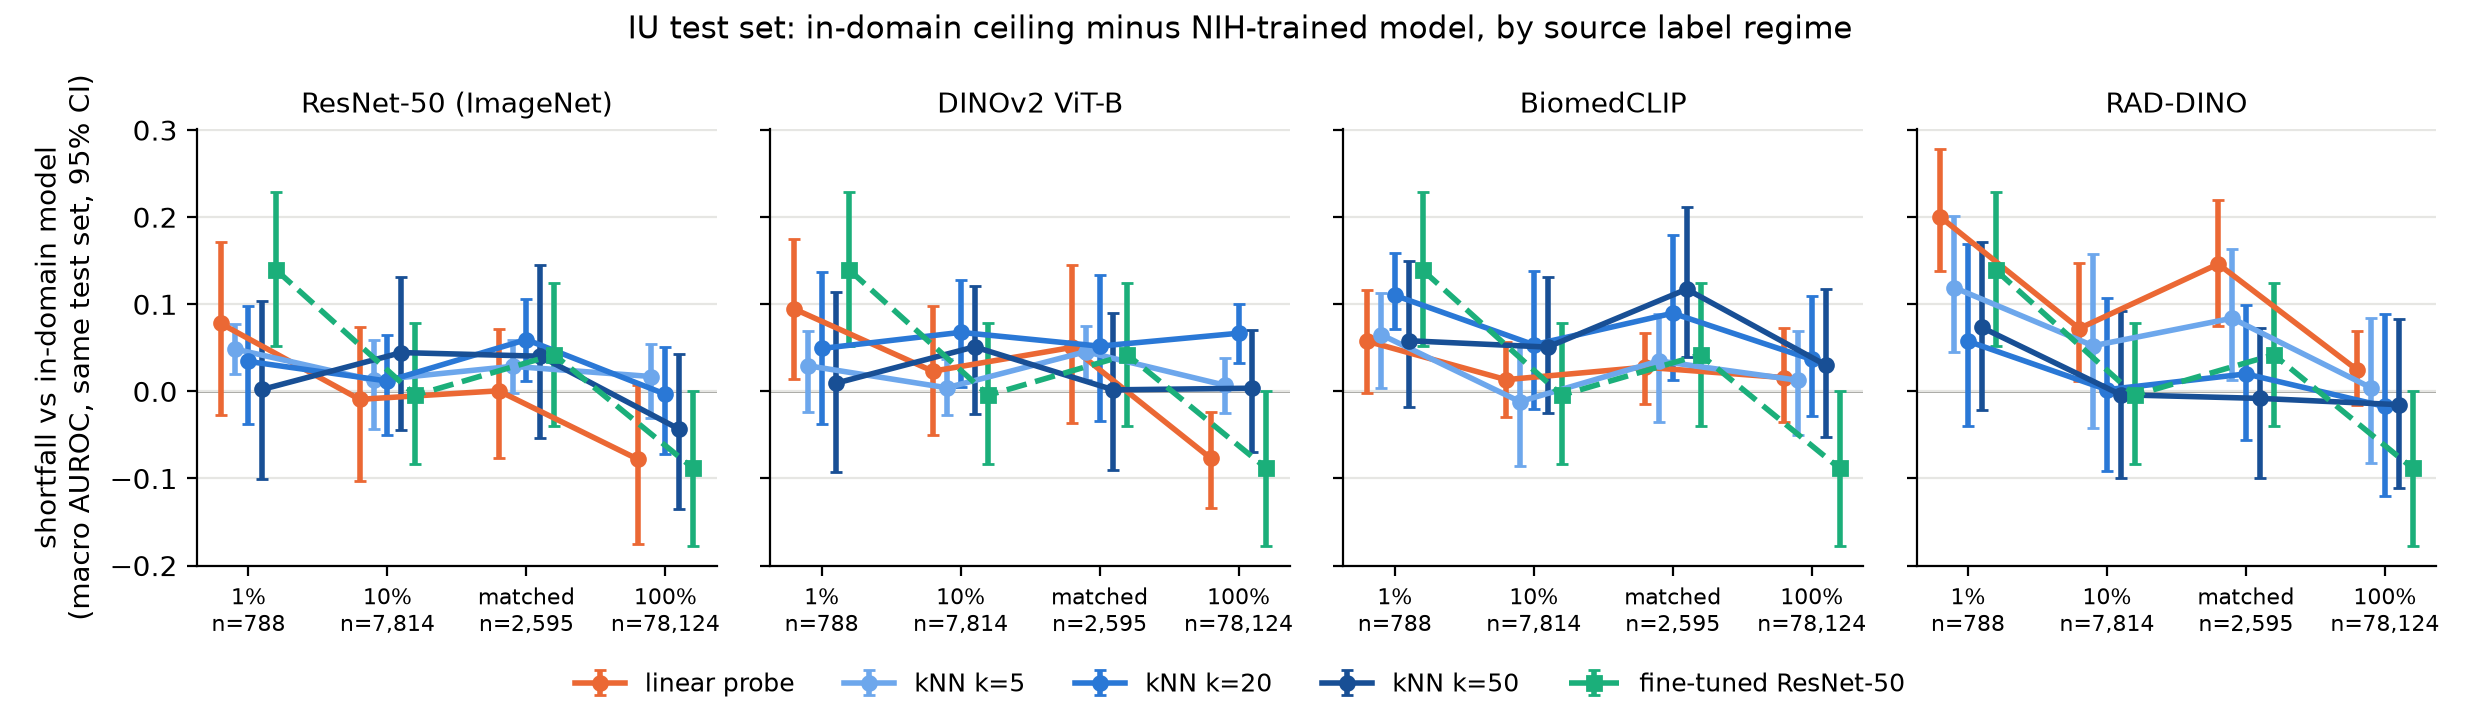
\includegraphics[width=\textwidth]{transfer_auroc_target_iu.png}
  \caption{Transfer gap by source label regime. Top: NIH test split, models trained on IU. Bottom: IU test split, models trained on NIH. Each panel is one frozen encoder; the dashed series is the fine-tuned ResNet-50, repeated in every panel as the baseline. Bars are 95\% paired patient-level bootstrap intervals.}
  \label{fig:transfer}
\end{figure*}

\section{Results}
\label{sec:results}

\subsection{Which gap?}
\label{sec:gapdef}
The protocol we set out with reports each model on its own test split (ID) and on the other dataset's test split (OOD) and calls ID~$-$~OOD the degradation. On these datasets that number is negative for most NIH-trained models: the ResNet-50 probe scores 0.714 on NIH and 0.826 on IU, the RAD-DINO probe 0.815 and 0.869 (Table~\ref{tab:idood}, appendix). IU's test split, hand-labelled and mostly normal, is simply an easier benchmark than NIH's official split, so a one-model-two-test-sets gap mixes shift with difficulty. We therefore fix the test set: on the target's test split, the \emph{transfer gap} is the in-domain model (trained on the target with all its labels) minus the source-trained model, evaluated on the same bootstrap resamples. Positive means the transferred model falls short of what in-domain training achieves.

\begin{table*}[!t]
  \caption{NIH test split, models trained on IU: transferred macro AUROC with, in parentheses, the gap to the in-domain ceiling (a model trained on NIH with all its labels) and, below it, the paired 95\% interval.}
  \label{tab:transfer_nih}
  \centering
  \begin{footnotesize}
\begin{tabular}{llcccc}
\toprule
encoder & head & ceiling & 1\% (26) & 10\% (259) & 100\% (2,594) \\
\midrule
ResNet-50 & probe & 0.714 & \begin{tabular}[t]{@{}c@{}}0.508 (+0.205)\\{\tiny[0.192, 0.217]}\end{tabular} & \begin{tabular}[t]{@{}c@{}}0.589 (+0.125)\\{\tiny[0.114, 0.136]}\end{tabular} & \begin{tabular}[t]{@{}c@{}}0.590 (+0.124)\\{\tiny[0.113, 0.134]}\end{tabular} \\
ResNet-50 & kNN$_{50}$ & 0.642 & \begin{tabular}[t]{@{}c@{}}0.500 (+0.142)\\{\tiny[0.133, 0.152]}\end{tabular} & \begin{tabular}[t]{@{}c@{}}0.574 (+0.069)\\{\tiny[0.058, 0.079]}\end{tabular} & \begin{tabular}[t]{@{}c@{}}0.567 (+0.075)\\{\tiny[0.063, 0.087]}\end{tabular} \\
DINOv2 & probe & 0.750 & \begin{tabular}[t]{@{}c@{}}0.537 (+0.213)\\{\tiny[0.203, 0.223]}\end{tabular} & \begin{tabular}[t]{@{}c@{}}0.596 (+0.155)\\{\tiny[0.143, 0.167]}\end{tabular} & \begin{tabular}[t]{@{}c@{}}0.628 (+0.123)\\{\tiny[0.114, 0.132]}\end{tabular} \\
DINOv2 & kNN$_{50}$ & 0.646 & \begin{tabular}[t]{@{}c@{}}0.500 (+0.146)\\{\tiny[0.137, 0.157]}\end{tabular} & \begin{tabular}[t]{@{}c@{}}0.561 (+0.085)\\{\tiny[0.075, 0.096]}\end{tabular} & \begin{tabular}[t]{@{}c@{}}0.554 (+0.092)\\{\tiny[0.082, 0.103]}\end{tabular} \\
BiomedCLIP & probe & 0.771 & \begin{tabular}[t]{@{}c@{}}0.592 (+0.179)\\{\tiny[0.171, 0.187]}\end{tabular} & \begin{tabular}[t]{@{}c@{}}0.679 (+0.091)\\{\tiny[0.083, 0.099]}\end{tabular} & \begin{tabular}[t]{@{}c@{}}0.696 (+0.075)\\{\tiny[0.067, 0.082]}\end{tabular} \\
BiomedCLIP & kNN$_{50}$ & 0.728 & \begin{tabular}[t]{@{}c@{}}0.500 (+0.228)\\{\tiny[0.219, 0.236]}\end{tabular} & \begin{tabular}[t]{@{}c@{}}0.666 (+0.062)\\{\tiny[0.054, 0.070]}\end{tabular} & \begin{tabular}[t]{@{}c@{}}0.678 (+0.050)\\{\tiny[0.042, 0.058]}\end{tabular} \\
RAD-DINO & probe & 0.815 & \begin{tabular}[t]{@{}c@{}}0.553 (+0.261)\\{\tiny[0.250, 0.271]}\end{tabular} & \begin{tabular}[t]{@{}c@{}}0.632 (+0.183)\\{\tiny[0.172, 0.193]}\end{tabular} & \begin{tabular}[t]{@{}c@{}}0.717 (+0.098)\\{\tiny[0.088, 0.107]}\end{tabular} \\
RAD-DINO & kNN$_{50}$ & 0.770 & \begin{tabular}[t]{@{}c@{}}0.500 (+0.270)\\{\tiny[0.261, 0.278]}\end{tabular} & \begin{tabular}[t]{@{}c@{}}0.627 (+0.143)\\{\tiny[0.131, 0.154]}\end{tabular} & \begin{tabular}[t]{@{}c@{}}0.698 (+0.072)\\{\tiny[0.063, 0.081]}\end{tabular} \\
ResNet-50 & fine-tuned & 0.814 & \begin{tabular}[t]{@{}c@{}}0.512 (+0.302)\\{\tiny[0.291, 0.314]}\end{tabular} & \begin{tabular}[t]{@{}c@{}}0.574 (+0.240)\\{\tiny[0.230, 0.250]}\end{tabular} & \begin{tabular}[t]{@{}c@{}}0.651 (+0.162)\\{\tiny[0.153, 0.171]}\end{tabular} \\
\bottomrule
\end{tabular}
\end{footnotesize}

\end{table*}

\begin{table*}[!t]
  \caption{IU test split, models trained on NIH, as in Table~\ref{tab:transfer_nih}; column headers give the number of source training images.}
  \label{tab:transfer_iu}
  \centering
  \begin{footnotesize}
\begin{tabular}{llccccc}
\toprule
encoder & head & ceiling & 1\% (788) & 10\% (7,814) & matched (2,595) & 100\% (78,124) \\
\midrule
ResNet-50 & probe & 0.748 & \begin{tabular}[t]{@{}c@{}}0.670 (+0.078)\\{\tiny[-0.027, 0.172]}\end{tabular} & \begin{tabular}[t]{@{}c@{}}0.757 (-0.009)\\{\tiny[-0.103, 0.074]}\end{tabular} & \begin{tabular}[t]{@{}c@{}}0.747 (+0.001)\\{\tiny[-0.077, 0.072]}\end{tabular} & \begin{tabular}[t]{@{}c@{}}0.826 (-0.078)\\{\tiny[-0.176, 0.007]}\end{tabular} \\
ResNet-50 & kNN$_{50}$ & 0.629 & \begin{tabular}[t]{@{}c@{}}0.627 (+0.002)\\{\tiny[-0.101, 0.104]}\end{tabular} & \begin{tabular}[t]{@{}c@{}}0.585 (+0.044)\\{\tiny[-0.045, 0.131]}\end{tabular} & \begin{tabular}[t]{@{}c@{}}0.589 (+0.040)\\{\tiny[-0.053, 0.145]}\end{tabular} & \begin{tabular}[t]{@{}c@{}}0.673 (-0.044)\\{\tiny[-0.135, 0.043]}\end{tabular} \\
DINOv2 & probe & 0.718 & \begin{tabular}[t]{@{}c@{}}0.623 (+0.095)\\{\tiny[0.014, 0.175]}\end{tabular} & \begin{tabular}[t]{@{}c@{}}0.695 (+0.023)\\{\tiny[-0.050, 0.098]}\end{tabular} & \begin{tabular}[t]{@{}c@{}}0.667 (+0.050)\\{\tiny[-0.036, 0.145]}\end{tabular} & \begin{tabular}[t]{@{}c@{}}0.795 (-0.077)\\{\tiny[-0.134, -0.024]}\end{tabular} \\
DINOv2 & kNN$_{50}$ & 0.607 & \begin{tabular}[t]{@{}c@{}}0.598 (+0.009)\\{\tiny[-0.092, 0.114]}\end{tabular} & \begin{tabular}[t]{@{}c@{}}0.556 (+0.051)\\{\tiny[-0.026, 0.121]}\end{tabular} & \begin{tabular}[t]{@{}c@{}}0.605 (+0.002)\\{\tiny[-0.090, 0.090]}\end{tabular} & \begin{tabular}[t]{@{}c@{}}0.604 (+0.004)\\{\tiny[-0.069, 0.071]}\end{tabular} \\
BiomedCLIP & probe & 0.848 & \begin{tabular}[t]{@{}c@{}}0.790 (+0.058)\\{\tiny[-0.002, 0.116]}\end{tabular} & \begin{tabular}[t]{@{}c@{}}0.835 (+0.013)\\{\tiny[-0.030, 0.057]}\end{tabular} & \begin{tabular}[t]{@{}c@{}}0.820 (+0.028)\\{\tiny[-0.015, 0.067]}\end{tabular} & \begin{tabular}[t]{@{}c@{}}0.832 (+0.016)\\{\tiny[-0.036, 0.072]}\end{tabular} \\
BiomedCLIP & kNN$_{50}$ & 0.760 & \begin{tabular}[t]{@{}c@{}}0.702 (+0.058)\\{\tiny[-0.018, 0.149]}\end{tabular} & \begin{tabular}[t]{@{}c@{}}0.710 (+0.051)\\{\tiny[-0.024, 0.131]}\end{tabular} & \begin{tabular}[t]{@{}c@{}}0.643 (+0.117)\\{\tiny[0.040, 0.212]}\end{tabular} & \begin{tabular}[t]{@{}c@{}}0.730 (+0.030)\\{\tiny[-0.053, 0.117]}\end{tabular} \\
RAD-DINO & probe & 0.893 & \begin{tabular}[t]{@{}c@{}}0.693 (+0.200)\\{\tiny[0.138, 0.278]}\end{tabular} & \begin{tabular}[t]{@{}c@{}}0.821 (+0.072)\\{\tiny[0.011, 0.147]}\end{tabular} & \begin{tabular}[t]{@{}c@{}}0.747 (+0.146)\\{\tiny[0.075, 0.220]}\end{tabular} & \begin{tabular}[t]{@{}c@{}}0.869 (+0.025)\\{\tiny[-0.016, 0.070]}\end{tabular} \\
RAD-DINO & kNN$_{50}$ & 0.801 & \begin{tabular}[t]{@{}c@{}}0.728 (+0.073)\\{\tiny[-0.022, 0.171]}\end{tabular} & \begin{tabular}[t]{@{}c@{}}0.805 (-0.004)\\{\tiny[-0.100, 0.092]}\end{tabular} & \begin{tabular}[t]{@{}c@{}}0.809 (-0.008)\\{\tiny[-0.100, 0.073]}\end{tabular} & \begin{tabular}[t]{@{}c@{}}0.817 (-0.015)\\{\tiny[-0.111, 0.083]}\end{tabular} \\
ResNet-50 & fine-tuned & 0.788 & \begin{tabular}[t]{@{}c@{}}0.649 (+0.139)\\{\tiny[0.052, 0.229]}\end{tabular} & \begin{tabular}[t]{@{}c@{}}0.793 (-0.004)\\{\tiny[-0.083, 0.078]}\end{tabular} & \begin{tabular}[t]{@{}c@{}}0.746 (+0.042)\\{\tiny[-0.039, 0.125]}\end{tabular} & \begin{tabular}[t]{@{}c@{}}0.877 (-0.088)\\{\tiny[-0.177, 0.001]}\end{tabular} \\
\bottomrule
\end{tabular}
\end{footnotesize}

\end{table*}

\subsection{Transfer to NIH from a small source}
Table~\ref{tab:transfer_nih} and the top row of Fig.~\ref{fig:transfer} show models trained on IU and tested on NIH. With all 2,594 IU images, the probes fall 0.075 (BiomedCLIP) to 0.124 (ResNet-50) AUROC short of their in-domain ceilings; the RAD-DINO probe reaches 0.717 against a ceiling of 0.815. Retrieval with $k=50$ falls 0.050 to 0.092 short ($k=5$ and $k=20$ are in the repository's results), and the paired contrast probe~$-$~$k$NN$_{50}$ is positive for every encoder (0.025 to 0.049, all intervals excluding zero). Retrieval does degrade less. It also starts lower: its in-domain ceilings are 0.04 to 0.07 below the probe's, and on the transferred numbers themselves the probe still beats $k$NN$_{50}$ for every encoder (e.g.\ RAD-DINO 0.717 vs 0.698). The fine-tuned ResNet-50 reaches 0.651 on NIH, a shortfall of 0.162 [0.153, 0.171] against its own 0.814 ceiling, larger than any frozen head (fine-tuned~$-$~probe 0.039 to 0.088; fine-tuned~$-$~$k$NN$_{50}$ 0.070 to 0.112, all paired intervals excluding zero). At 1\% of IU (26 images) every model is within 0.1 AUROC of chance.

\subsection{Transfer to IU from a large source}
Table~\ref{tab:transfer_iu} and the bottom row of Fig.~\ref{fig:transfer} reverse the direction. With all 78,124 NIH images, the NIH-trained probes match or beat the IU-trained ceilings for three encoders (gaps $-0.078$, $-0.077$ and $0.016$ for ResNet-50, DINOv2 and BiomedCLIP) and come within interval of it for RAD-DINO (0.025 [$-0.016$, 0.070]); the fine-tuned network does the same (0.877 vs an IU-trained ceiling of 0.788). Source label count, not hospital, dominates here. The matched regime makes the point: with 2,594 NIH images the probe gaps are 0.001, 0.050 and 0.028 for the three weaker encoders, but 0.146 [0.075, 0.220] for RAD-DINO, whose in-domain IU probe profits most from IU's cleaner labels. RAD-DINO retrieval at matched size transfers with no loss ($k$NN$_{50}$ gap $-0.008$), and the paired contrast probe~$-$~$k$NN$_{50}$ is 0.154 [0.053, 0.254]: the one setting where retrieval both degrades less and ends higher (0.809 vs 0.747).


\subsection{Label regimes in-domain}
On NIH's own test split, the fine-tuned ResNet-50 trails the RAD-DINO probe by 0.109 AUROC at 1\% of the labels (0.580 vs 0.689), 0.086 at 10\% (0.692 vs 0.778) and 0.116 at the matched size (0.630 vs 0.746), and ties it at 100\% (0.814 [0.807, 0.821] vs 0.815 [0.808, 0.822]). The frozen-encoder advantage is a small-data advantage. The ordering of the frozen encoders is stable across regimes: ImageNet ResNet-50 (0.714 at 100\%) $<$ DINOv2 (0.750) $<$ BiomedCLIP (0.771) $<$ RAD-DINO (0.815).

\subsection{Calibration}
IU-trained models are poorly calibrated on NIH, whichever head: probe ECE rises from 0.013--0.022 in-domain to 0.066--0.120 on NIH, and the fine-tuned network from 0.018 to 0.103, consistent with the prevalence shift between the two populations. NIH-trained models stay near 0.03 on IU. In-domain, $k$NN with $k=5$ is the worst-calibrated head (ECE 0.07--0.09) because its scores take only six values. ECE on IU's rare labels is dominated by prevalence; we treat AUROC as the primary metric.

\begin{figure}[!t]
  \centering
  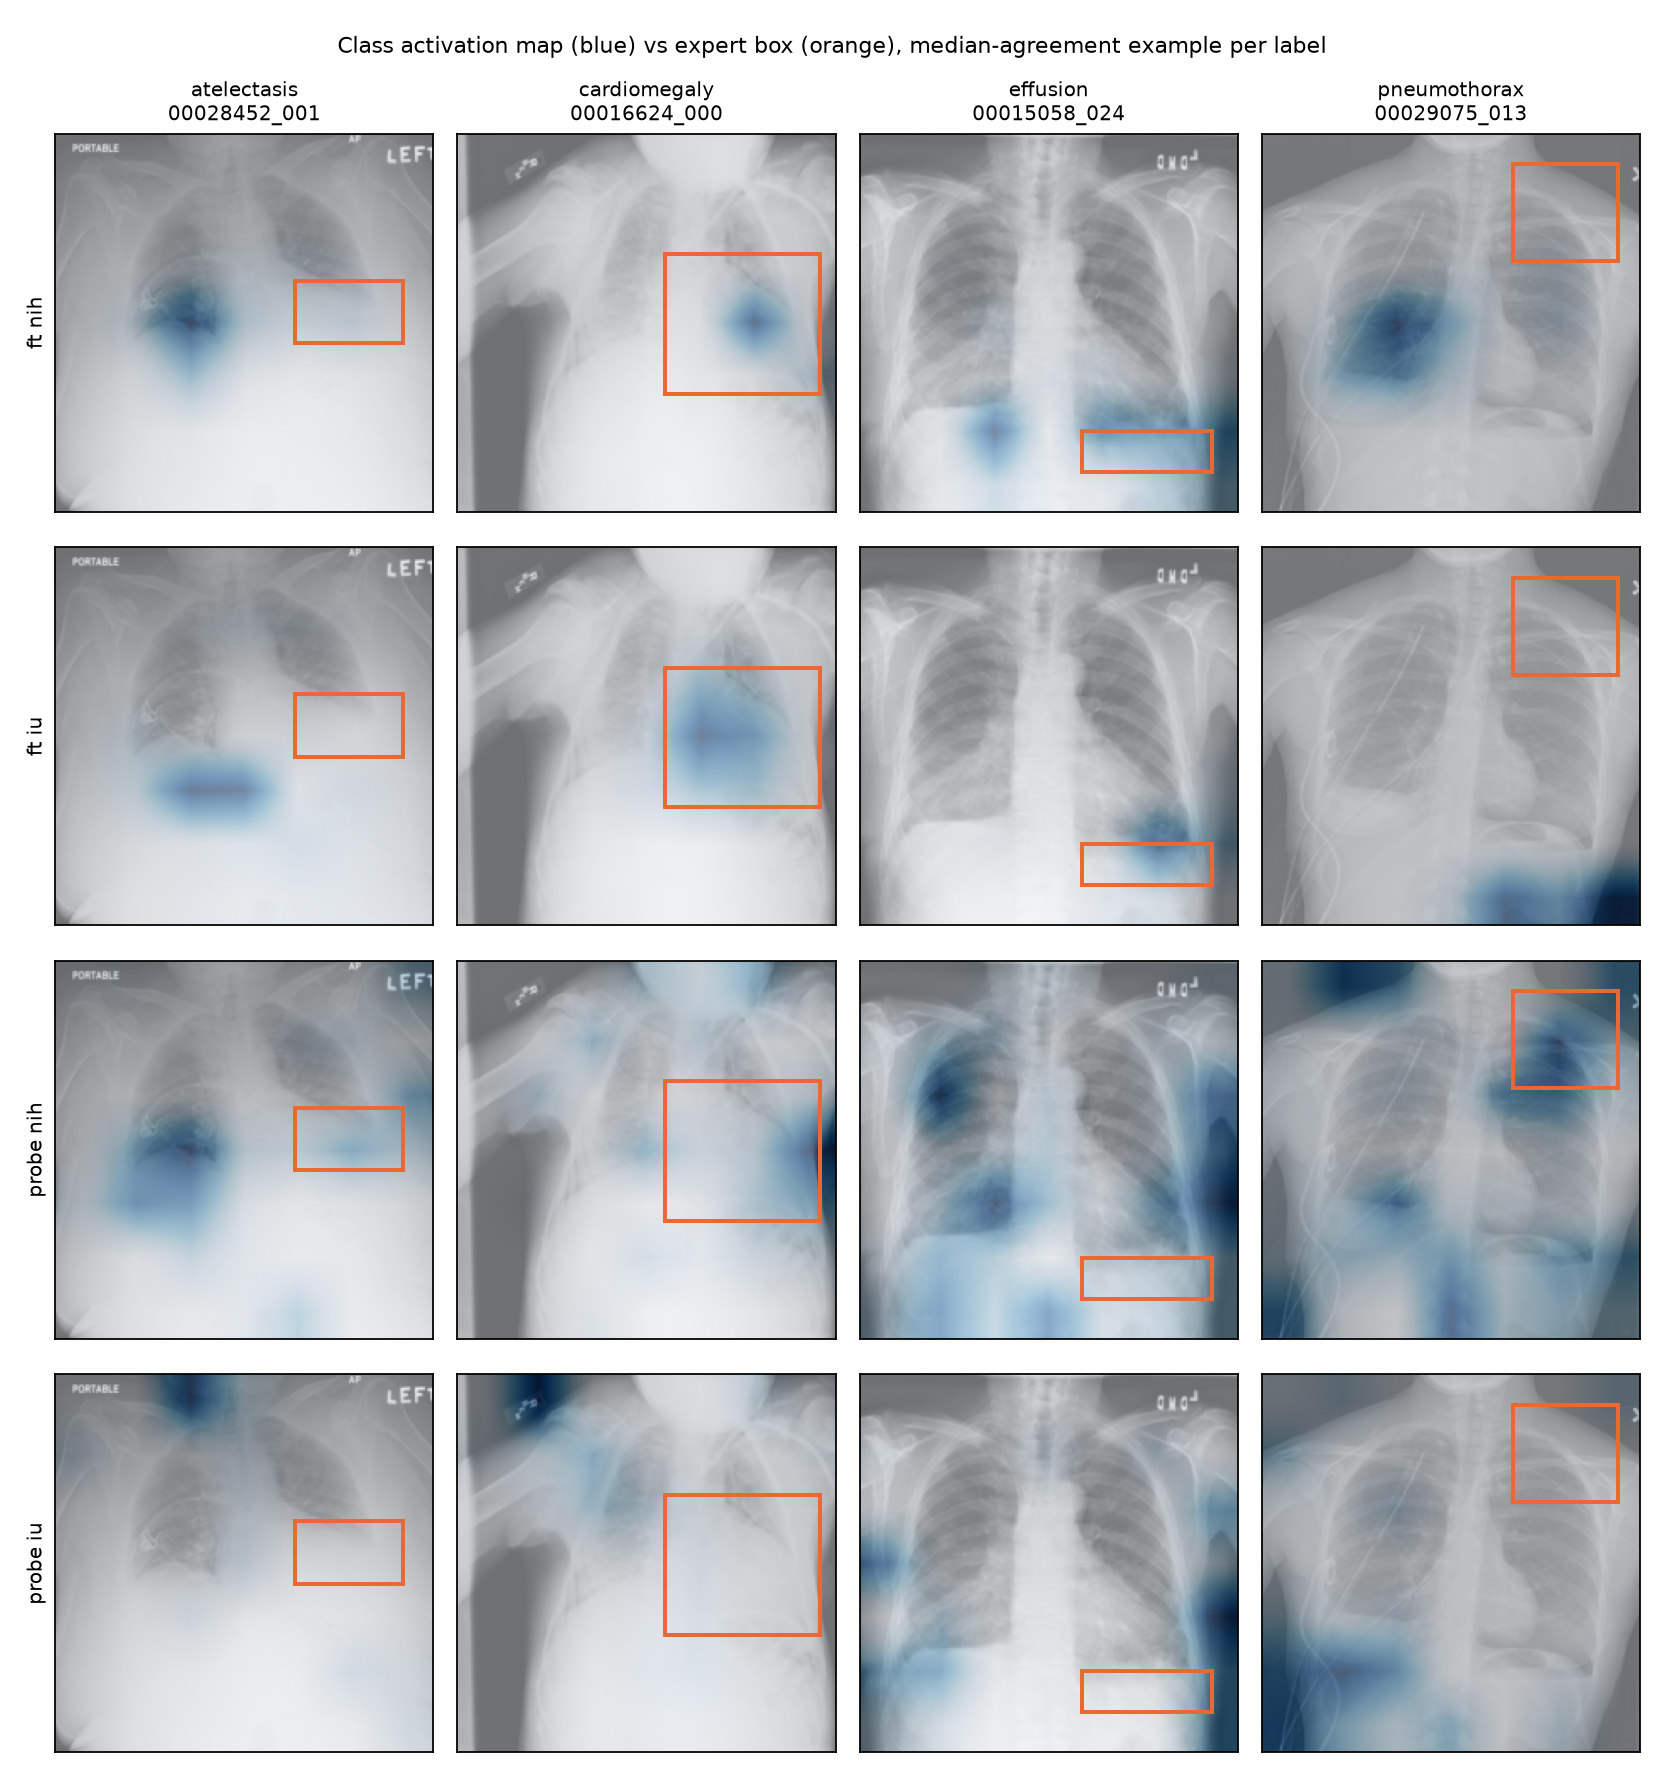
\includegraphics[width=\columnwidth]{gradcam_examples.png}
  \caption{Class activation map (blue) and expert box (orange) for the box with median energy agreement per label, for each of the four models.}
  \label{fig:cam}
\end{figure}

\subsection{Localisation}
Table~\ref{tab:gradcam} scores the class activation maps against the radiologist boxes. The NIH-trained fine-tuned network puts its maximum inside the box for 44.5\% of boxes [40.2, 49.2] against a chance level of 10.8\%, driven by cardiomegaly (93.4\%); pneumothorax stays at chance (9.7\% vs 7.0\%). The frozen ResNet-50 with the NIH probe reaches 22.2\%; the paired gain from fine-tuning is 0.223 [0.178, 0.269]. Trained on IU and scored on the same NIH images, the fine-tuned network drops to 33.9\% (paired $-0.105$ [$-0.144$, $-0.069$]), still above either frozen probe; cardiomegaly transfers (89.0\%) while atelectasis collapses (32.5\% to 11.1\%). Fig.~\ref{fig:cam} shows the median-agreement box per label rather than a selected success.

\begin{table*}[!t]
  \caption{Class activation maps vs 576 expert boxes on the NIH test split. Pointing: the map maximum falls inside the box (the pointing game); energy: fraction of map mass inside the box; brackets are paired 95\% patient-level bootstrap intervals. The last row is what a uniform map scores.}
  \label{tab:gradcam}
  \centering
  \begin{footnotesize}
\begin{tabular}{lcccccc}
\toprule
& & & \multicolumn{4}{c}{pointing game per label} \\
\cmidrule(lr){4-7}
model & pointing & energy & atelectasis & cardiomegaly & effusion & pneumothorax \\
\midrule
FT, NIH-trained & \begin{tabular}[t]{@{}c@{}}0.445\\{\tiny[0.402, 0.492]}\end{tabular} & \begin{tabular}[t]{@{}c@{}}0.345\\{\tiny[0.313, 0.378]}\end{tabular} & 0.325 & 0.934 & 0.340 & 0.097 \\
FT, IU-trained & \begin{tabular}[t]{@{}c@{}}0.339\\{\tiny[0.296, 0.384]}\end{tabular} & \begin{tabular}[t]{@{}c@{}}0.275\\{\tiny[0.243, 0.307]}\end{tabular} & 0.111 & 0.890 & 0.255 & 0.067 \\
frozen, NIH probe & \begin{tabular}[t]{@{}c@{}}0.222\\{\tiny[0.187, 0.258]}\end{tabular} & \begin{tabular}[t]{@{}c@{}}0.157\\{\tiny[0.141, 0.171]}\end{tabular} & 0.100 & 0.466 & 0.190 & 0.134 \\
frozen, IU probe & \begin{tabular}[t]{@{}c@{}}0.160\\{\tiny[0.130, 0.192]}\end{tabular} & \begin{tabular}[t]{@{}c@{}}0.134\\{\tiny[0.120, 0.148]}\end{tabular} & 0.067 & 0.322 & 0.170 & 0.072 \\
\midrule
chance (uniform map) & 0.108 & 0.108 & 0.043 & 0.233 & 0.090 & 0.070 \\
\bottomrule
\end{tabular}
\end{footnotesize}

\end{table*}

\section{Discussion and limitations}

Three answers come out of the grid. First, the one-model-two-test-sets gap is not a measure of robustness on these datasets: it is negative for most NIH-trained models because the hand-labelled IU split is the easier benchmark, and only a same-test-set comparison against an in-domain model, on the same bootstrap resamples, separates the hospital effect from the benchmark effect. Second, retrieval over a frozen index degrades less than a linear probe when the source is small, for every encoder, but it starts from a lower ceiling, and in most cells the probe is still the better transferred model. The exception is the configuration a small site would actually run: RAD-DINO retrieval built from 2,594 NIH images transfers to IU with no measurable loss (gap $-0.008$) and ends above the probe there (0.809 vs 0.747). Third, the advantage of frozen medical encoders over end-to-end fine-tuning is a small-data advantage. With 2.6k source labels the fine-tuned ResNet-50 trails the RAD-DINO probe by 0.07 to 0.12 AUROC and shows the largest transfer shortfall of any model; with 78k labels it ties the best frozen pipeline in domain and out of domain, and its activation maps land on the radiologist's box twice as often as the frozen probe's. A site choosing between the two workflows should count its labels first.

Several confounds limit what these numbers mean. IU's labels are manual MeSH terms and NIH's are report-mined, so every cross-dataset number mixes label-definition shift with image shift; the collapse of atelectasis localisation under IU training (32.5\% to 11.1\%) may be as much about what IU calls atelectasis as about the images. RAD-DINO saw every NIH image during pretraining, so its NIH numbers are not clean in-distribution estimates, and IU-as-target is the only direction unseen by every encoder. IU is small, with five consolidation and six pneumothorax positives in its test split and no patient identifiers, so its intervals are wide and its ``patients'' are reports. VinDr-CXR, CheXpert and MIMIC-CXR would strengthen the study but require credentialed access we did not use. Only one fine-tuned architecture and one recipe were run; point estimates come from a single seed, with the spread over three seeds reported in the repository; and calibration was measured without any post-hoc recalibration. None of this is a clinical evaluation, and no clinical utility is claimed: the question studied is which workflow holds up when the images come from a different hospital, not whether either should be used on patients.

\paragraph{Reproducibility}
Code, label mapping, split files, cached embeddings and every table and figure are regenerated by a single command from the repository at \url{https://github.com/xeij/medical-vision}; the fine-tuning grid (17 runs) is resumable and took 7.6 hours on a laptop GPU.

\begin{table*}[!t]
  \caption{Macro AUROC at 100\% labels on each model's own test split (ID) and the other dataset's test split (OOD), with ID~$-$~OOD and its 95\% interval. Negative values in the NIH-trained block show the test-split difficulty confound of Section~\ref{sec:gapdef}.}
  \label{tab:idood}
  \centering
  \begin{footnotesize}
\begin{tabular}{llcccccc}
\toprule
& & \multicolumn{3}{c}{trained on NIH} & \multicolumn{3}{c}{trained on IU} \\
\cmidrule(lr){3-5} \cmidrule(lr){6-8}
encoder & head & ID & OOD & ID $-$ OOD & ID & OOD & ID $-$ OOD \\
\midrule
ResNet-50 & probe & 0.714 & 0.826 & \begin{tabular}[t]{@{}c@{}}-0.112\\{\tiny[-0.170, -0.027]}\end{tabular} & 0.748 & 0.590 & \begin{tabular}[t]{@{}c@{}}+0.158\\{\tiny[0.082, 0.233]}\end{tabular} \\
ResNet-50 & kNN$_{5}$ & 0.558 & 0.541 & \begin{tabular}[t]{@{}c@{}}+0.017\\{\tiny[-0.029, 0.052]}\end{tabular} & 0.558 & 0.524 & \begin{tabular}[t]{@{}c@{}}+0.034\\{\tiny[0.010, 0.058]}\end{tabular} \\
ResNet-50 & kNN$_{20}$ & 0.614 & 0.598 & \begin{tabular}[t]{@{}c@{}}+0.016\\{\tiny[-0.059, 0.067]}\end{tabular} & 0.595 & 0.548 & \begin{tabular}[t]{@{}c@{}}+0.046\\{\tiny[0.016, 0.078]}\end{tabular} \\
ResNet-50 & kNN$_{50}$ & 0.642 & 0.673 & \begin{tabular}[t]{@{}c@{}}-0.031\\{\tiny[-0.106, 0.049]}\end{tabular} & 0.629 & 0.567 & \begin{tabular}[t]{@{}c@{}}+0.062\\{\tiny[0.011, 0.124]}\end{tabular} \\
DINOv2 & probe & 0.750 & 0.795 & \begin{tabular}[t]{@{}c@{}}-0.044\\{\tiny[-0.118, 0.045]}\end{tabular} & 0.718 & 0.628 & \begin{tabular}[t]{@{}c@{}}+0.090\\{\tiny[0.007, 0.173]}\end{tabular} \\
DINOv2 & kNN$_{5}$ & 0.564 & 0.534 & \begin{tabular}[t]{@{}c@{}}+0.030\\{\tiny[0.004, 0.053]}\end{tabular} & 0.541 & 0.524 & \begin{tabular}[t]{@{}c@{}}+0.017\\{\tiny[-0.007, 0.043]}\end{tabular} \\
DINOv2 & kNN$_{20}$ & 0.617 & 0.546 & \begin{tabular}[t]{@{}c@{}}+0.071\\{\tiny[0.017, 0.113]}\end{tabular} & 0.613 & 0.543 & \begin{tabular}[t]{@{}c@{}}+0.069\\{\tiny[0.026, 0.121]}\end{tabular} \\
DINOv2 & kNN$_{50}$ & 0.646 & 0.604 & \begin{tabular}[t]{@{}c@{}}+0.043\\{\tiny[-0.035, 0.114]}\end{tabular} & 0.607 & 0.554 & \begin{tabular}[t]{@{}c@{}}+0.053\\{\tiny[0.011, 0.109]}\end{tabular} \\
BiomedCLIP & probe & 0.771 & 0.832 & \begin{tabular}[t]{@{}c@{}}-0.062\\{\tiny[-0.115, -0.001]}\end{tabular} & 0.848 & 0.696 & \begin{tabular}[t]{@{}c@{}}+0.152\\{\tiny[0.098, 0.199]}\end{tabular} \\
BiomedCLIP & kNN$_{5}$ & 0.619 & 0.636 & \begin{tabular}[t]{@{}c@{}}-0.017\\{\tiny[-0.085, 0.036]}\end{tabular} & 0.649 & 0.612 & \begin{tabular}[t]{@{}c@{}}+0.036\\{\tiny[0.008, 0.063]}\end{tabular} \\
BiomedCLIP & kNN$_{20}$ & 0.694 & 0.715 & \begin{tabular}[t]{@{}c@{}}-0.021\\{\tiny[-0.105, 0.061]}\end{tabular} & 0.752 & 0.661 & \begin{tabular}[t]{@{}c@{}}+0.091\\{\tiny[0.025, 0.161]}\end{tabular} \\
BiomedCLIP & kNN$_{50}$ & 0.728 & 0.730 & \begin{tabular}[t]{@{}c@{}}-0.003\\{\tiny[-0.091, 0.087]}\end{tabular} & 0.760 & 0.678 & \begin{tabular}[t]{@{}c@{}}+0.083\\{\tiny[0.017, 0.151]}\end{tabular} \\
RAD-DINO & probe & 0.815 & 0.869 & \begin{tabular}[t]{@{}c@{}}-0.054\\{\tiny[-0.110, 0.017]}\end{tabular} & 0.893 & 0.717 & \begin{tabular}[t]{@{}c@{}}+0.176\\{\tiny[0.139, 0.211]}\end{tabular} \\
RAD-DINO & kNN$_{5}$ & 0.654 & 0.707 & \begin{tabular}[t]{@{}c@{}}-0.052\\{\tiny[-0.126, 0.015]}\end{tabular} & 0.711 & 0.625 & \begin{tabular}[t]{@{}c@{}}+0.086\\{\tiny[0.028, 0.160]}\end{tabular} \\
RAD-DINO & kNN$_{20}$ & 0.737 & 0.767 & \begin{tabular}[t]{@{}c@{}}-0.030\\{\tiny[-0.100, 0.051]}\end{tabular} & 0.750 & 0.674 & \begin{tabular}[t]{@{}c@{}}+0.075\\{\tiny[0.012, 0.147]}\end{tabular} \\
RAD-DINO & kNN$_{50}$ & 0.770 & 0.817 & \begin{tabular}[t]{@{}c@{}}-0.047\\{\tiny[-0.107, 0.033]}\end{tabular} & 0.801 & 0.698 & \begin{tabular}[t]{@{}c@{}}+0.104\\{\tiny[0.036, 0.168]}\end{tabular} \\
ResNet-50 & fine-tuned & 0.814 & 0.877 & \begin{tabular}[t]{@{}c@{}}-0.063\\{\tiny[-0.109, 0.005]}\end{tabular} & 0.788 & 0.651 & \begin{tabular}[t]{@{}c@{}}+0.137\\{\tiny[0.075, 0.200]}\end{tabular} \\
\bottomrule
\end{tabular}
\end{footnotesize}

\end{table*}

\appendix[The gap as specified]
Table~\ref{tab:idood} reports the degradation as the protocol originally defined it, one model evaluated on its own test split and on the other dataset's, for every encoder and head at 100\% of the source labels.

\bibliographystyle{IEEEtran}
\bibliography{refs}


\end{document}
